
\documentclass[12pt,a4]{article}

\usepackage[utf8]{inputenc}
\usepackage[T1]{fontenc}
\usepackage{amsmath, amssymb, amsfonts}
\usepackage{mathtools}
\usepackage{graphicx, float, epstopdf}
\usepackage{enumerate}
\usepackage{bm}
\usepackage[noabbrev]{cleveref}
\DeclareMathOperator*{\argmin}{\arg\!\min}

\newcommand{\R}{{\mathbb R}}
\newcommand{\C}{{\mathbb C}}
\newcommand{\N}{{\mathbb N}}
\newcommand{\ra}{\rightarrow}
\newcommand{\lra}{\longrightarrow}
\newcommand{\lnorm}{\left\|}
\newcommand{\rnorm}{\right\|}
\newcommand{\ind}{{\mathbf{1}}}

\newcommand{\citeneeded}{\ensuremath{\vphantom{1}^{\text{[citation needed]}}\,}}
\newcommand{\eps}{\ensuremath{\varepsilon}}
\newcommand{\vc}[1]{\ensuremath{\bm{#1}}}
\newcommand*{\bigCI}{%
  \mathrel{\text{%
    {\rotatebox[origin=c]{90}{\resizebox{2.25ex}{1.65ex}{$\vDash$}}}%
  }}%
}

\title{Expected value of the norm of a random variable that follows a multivariate normal distribution with zero mean}
\author{Lasse Lybeck, Robert Sirviö}


\begin{document}

\maketitle

\section{Introduction}

In this work we will discuss the expected value of the norm of a random variable that follows a multivariate normal distribution with zero mean. More precisely, we will study the claim in \cite{samu}, section 5.4.1 (p. 72), which states, that if the noise vector is a sample of $\eps \in \R^k$ where $\eps_j \sim N(0, \sigma^2)$, then the expected value satisfies $E \left( \lnorm \eps \rnorm \right) = \sqrt{k} \sigma$. We will see that this claim is imprecise. It turns out however, that the statement is \emph{asymptotically} true, and that the convergence toward the precise result is very fast.

\section{Calculations}
\label{sec:calc}


\subsection{Analytical}
\label{sec:analytical}
Let
\begin{equation}
\vc{\eps'} = \left(Z_1, \ldots, Z_n \right), \quad Z_i \sim N(0,1) \bigCI \text{ for all }
i \in \left\{1, \ldots, n\right\} 
\end{equation}
and define
\begin{equation}
\label{eq:epsdef}
\vc{\eps} := \sigma \vc{\eps'} = \left(\sigma Z_1, \ldots, \sigma Z_n \right), \quad \sigma > 0.
\end{equation}
Now it holds that
\begin{equation}
\sigma Z_i \sim N\left(0,\sigma^2\right) \text{ for all }
i \in \left\{1, \ldots, n\right\}.
\end{equation}

Let now $X \sim \chi_n^2$ and $Y \sim \chi_n$, where $\chi_n^2$ denotes the chi-squared distribution and $\chi_n$ the chi distribution, both with $n$ degrees of freedom. We now see (\cite{handbook}, \cite{chi}, \cite{mathworld}) that
\begin{equation}
\label{eq:calc}
\begin{alignedat}{1}
E\left(\lnorm \vc{\eps} \rnorm \right)   &= E\left(\lnorm \sigma \vc{\eps'} \rnorm \right)   =
E\left(\sigma \lnorm \vc{\eps'} \rnorm \right) = \sigma E\left(\lnorm \vc{\eps'} \rnorm \right) \\
&= \sigma E\left(\sqrt{Z_1^2 + \ldots + Z_n^2} \right) = \sigma E\left(\sqrt{X} \right) \\
&= \sigma E\left( Y \right) = 
\sigma \sqrt{2}\frac{\Gamma\left(\frac{n+1}{2}\right)}{\Gamma\left(\frac{n}{2}\right)} \\
&= \sigma \sqrt{2} \sqrt{\frac{n}{2}} \left( 1 - \frac{1}{80 n/2} + \frac{1}{128 (n/2)^2} + \frac{5}{1024 (n/2)^3} \right. \\ & \qquad \qquad \qquad \qquad \left. - \frac{21}{32768 (n/2)^4} + O\left( n^{-5} \right) \right) \\
&= \sigma \sqrt{n} \left( 1 - \frac{1}{4 n} + \frac{1}{32 n^2} + \frac{5}{128 n^3} - \frac{21}{2048 n^4} + O\left( n^{-5} \right) \right) .
\end{alignedat}
\end{equation}

\subsection{Numerical}
\label{sec:numerical}
We also simulated the setting with MATLAB by comparing the the different expressions of the expected value and further increasing the dimension of multivariate normal distribution. These results can be seen in \cref{fig:err}.
\begin{figure}[H]
\begin{center}
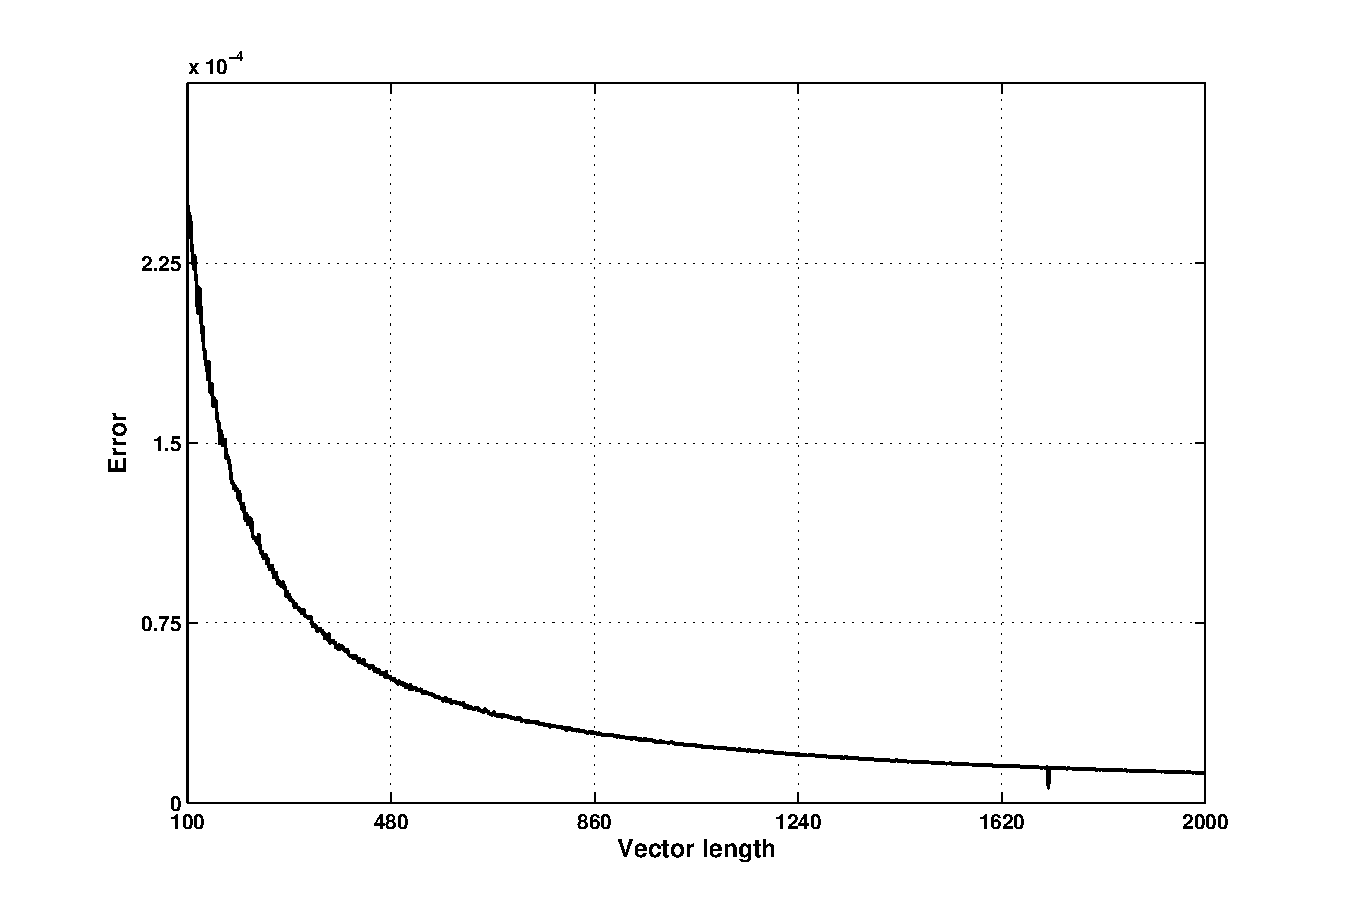
\includegraphics[scale=.4]{img/exp_val_simulation.eps}
\end{center}
\caption{The difference between the two expressions of the expected value.}
\label{fig:err}
\end{figure}
The validity of the analytically acquired expression of the expected value was verified by computing the norm of a vector of predefined dimension with elements originating from a normal distribution with zero mean and a fixed variance. These results can be seen in \cref{fig:errTarget}.
\begin{figure}[H]
\begin{center}
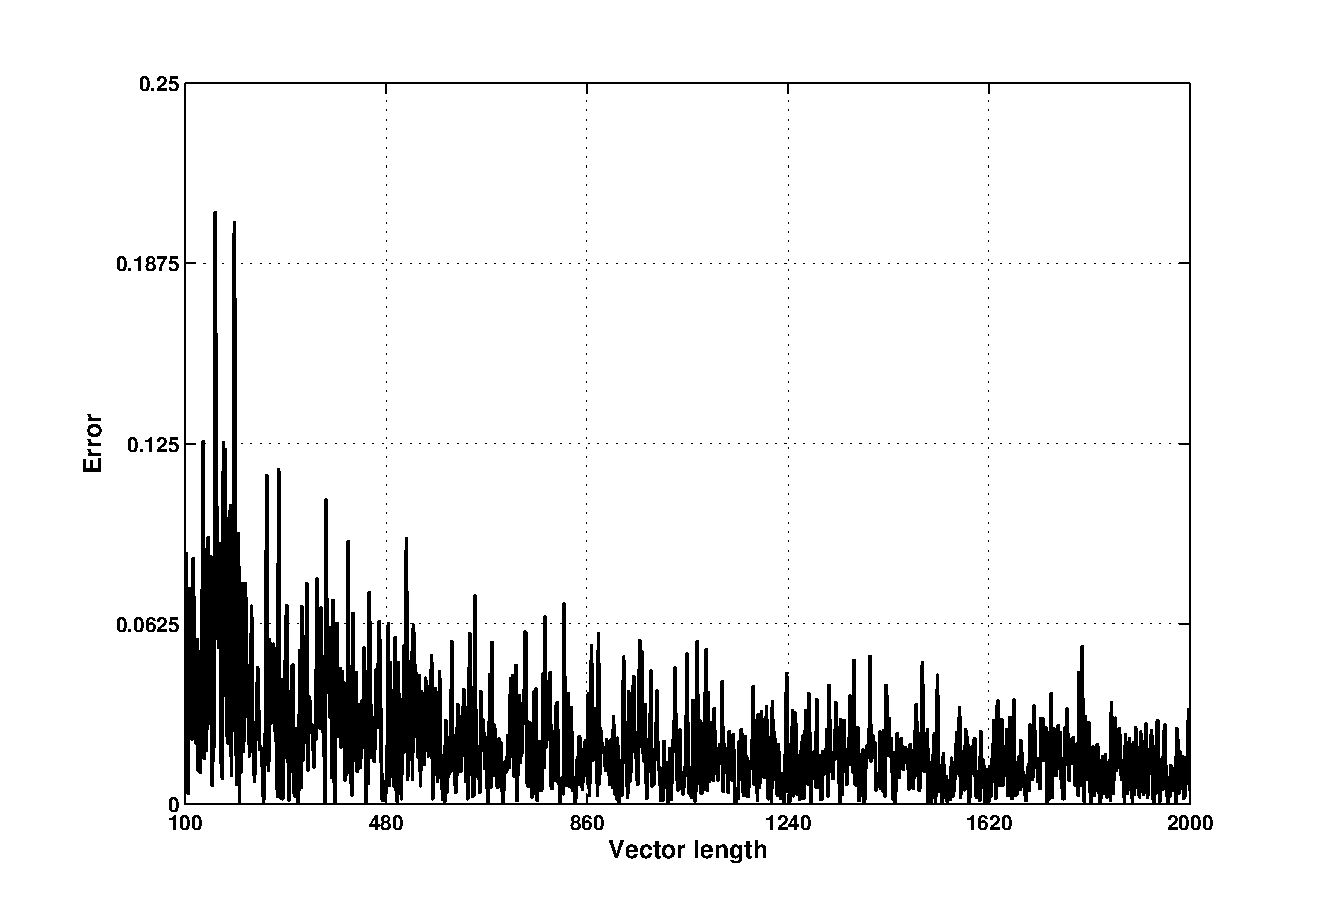
\includegraphics[scale=.5]{img/exp_val_simulation_targetErr.eps}
\end{center}
\caption{The difference norm of the target vector and the analytically acquired expression of the expected value.}
\label{fig:errTarget}
\end{figure}

\section{Discussion}

As we can see from \cref{eq:calc} in \cref{sec:calc}, it is clear that for every $n > 0$ and $\eps$ as defined in \cref{eq:epsdef} we get
\begin{equation}
E \left( \lnorm \eps \rnorm \right) < \sigma \sqrt{n} .
\end{equation}
However, it is also easy to see that 
\begin{equation}
\lim_{n \rightarrow \infty} E \left( \lnorm \eps \rnorm \right) = \sigma \sqrt{n} .
\end{equation}


%----------------------References---------------------
%\newpage
\begin{thebibliography}{9}

\begin{footnotesize}
    
\bibitem{handbook}
    Abramowitz, M \& Stegun, I.A. (1965)
    \emph{Handbook of mathematical functions with formulas, graphs and mathenatical tables}
    New York, NY: Dover, p. 940
    
\bibitem{chi}
    Evans, M., Hastings, N. \& Peacock, B. (2000)
    \emph{Statistical distributions}.
    New York: Wiley, p. 57
    
\bibitem{samu}
	Mueller, Jennifer L. \& Siltanen Samuli, (2012).
	\emph{Linear and Nonlinear Inverse Problems with Practical Applications}.
	SIAM, 1st edition.

\bibitem{mathworld}
    http://mathworld.wolfram.com/GammaFunction.html. Wolfram Mathworld: Gamma Function, equation (98). Last accessed 9th May 2014.


\end{footnotesize}

\end{thebibliography}

\end{document}



